\documentclass[xcolor=pdftex,dvipsnames,table,mathserif]{beamer}
\usepackage{subfigure}
\usepackage{amsbsy}
\usepackage{tikz}
\usetikzlibrary{arrows}
\usepackage{amsmath,graphicx,dsfont,color}
\usepackage{amsfonts}
\usepackage{amssymb}
\usepackage{array}

\bibliographystyle{apalike}

\setbeamertemplate{bibliography item}{\insertbiblabel}
\setbeamertemplate{bibliography entry title}{}
\setbeamertemplate{bibliography entry location}{}
\setbeamertemplate{bibliography entry note}{}

%Definitiona

\newcommand{\x}{\mathbf{x}}
\newcommand{\X}{\mathbf{X}}
\newcommand{\W}{\mathbf{W}} %Weight
\newcommand{\bais}{\mathbf{b}}%Bais
\newcommand{\act}{\texttt{g}}%Activation
\newcommand{\loss}{L}
\newcommand{\pdata}{\hat{p}_{\texttt{data}}}
\newcommand{\nsize}{n}
\newcommand{\param}{\boldsymbol{\theta}}
\newcommand{\featmap}{\boldsymbol{\phi}}
\newcommand{\EV}{\mathbb{E}}







\usepackage{physics}

\graphicspath{{../graphics/}}

%% \usepackage{animate}

\AtBeginSection[]{
  \begin{frame}{Contents}
  \tableofcontents[currentsection, hideothersubsections]
  \end{frame}
}

\AtBeginSubsection[]{
  \begin{frame}{Contents}
  \tableofcontents[currentsection, subsectionstyle=show/shaded/hide]
  \end{frame}
}

\setbeamertemplate{footline}[frame number]{}
\setbeamertemplate{navigation symbols}{}
\setbeamertemplate{section in toc}[square]
\setbeamertemplate{items}[square]

\title{Deep Learning for Image Analysis\\Course Introduction}
\author{E. Decencière, Thomas Walter, Santiago Velasco-Forero}
\date{Mines Paris\\
  PSL Research University
}
\titlegraphic{
\includegraphics[height=1.7cm]{../graphics/logoemp}}

\useinnertheme{rounded}
\usecolortheme{rose}

%%%%%%%%%%%%%%%%%%%%%%%%%%%%%%%%%%%%%%%%%%%%%%%%%%
%%%%%%%%%%%%%%%%%%%%%%%%%%%%%%%%%%%%%%%%%%%%%%%%%%
\begin{document}
\begin{frame}
\titlepage
\end{frame}

%%%%%%%%%%%%%%%%%%%%%%%%%%%%%%%%%%%%
\begin{frame}{Course language}

\begin{itemize}
\item Course material (slides, notebooks, etc.) in English
\item Oral language: TBD
\end{itemize}

\end{frame}



%%%%%%%%%%%%%%%%%%%%%%%%%%%%%%%%%%%%%%%%%%%%%%%%%%
\frame{
  \frametitle{About the lecturers}

\begin{columns}
  \begin{column}{.2\textwidth}
\vfill
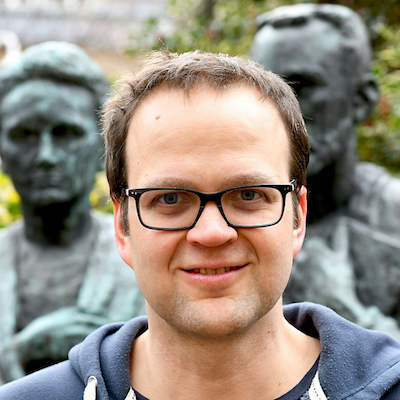
\includegraphics[width=\textwidth]{ThomasWalter.jpg}\\
\vspace{2em}
    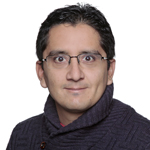
\includegraphics[width=\textwidth]{velascoforero}\\
\vspace{2em}
    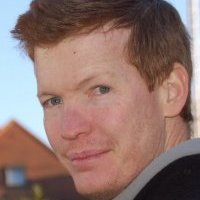
\includegraphics[width=\textwidth]{ed.jpg}

  \end{column}
  \begin{column}{.8\textwidth}

    \begin{block}{Thomas Walter}
      \scriptsize{
    \begin{itemize}
    \item Researcher on bioimage informatics, director of the Centre for Computational Biology (CBIO)
    \item Main application fields: Biology, medicine
    \end{itemize}
    }
  \end{block}

  \begin{block}{Santiago Velasco-Forero}
      \scriptsize{
    \begin{itemize}
    \item Researcher on image processing, pattern recognition, multivariate statistics, graph-based data/image analysis
    \item Main application fields: Remote Sensing, cosmetology, astronomy, hyperspectral imaging.
    \end{itemize}
    }
  \end{block}

    \begin{block}{Etienne Decencière}
      \scriptsize{
    \begin{itemize}
    \item Researcher on image analysis, mathematical morphology, deep learning; director of the Center for Mathematical Morphology
    \item Main application fields: biometry, dermatology, materials science
    \end{itemize}
    }
  \end{block}

  \end{column}
\end{columns}

}

%%%%%%%%%%%%%%%%%%%%%%%%%%%%%%%%%%%%
\begin{frame}{Course organization}

  \begin{block}{Communication}


    \begin{itemize}
      \item Microsoft Teams
      \begin{itemize}
      \item Announcements
      \item Questions about course and practical sessions
      \end{itemize}
    \item E-mail
      \begin{itemize}
      \item General organization, absence justification: Etienne.Decenciere@minesparis.psl.eu
      \end{itemize}
    \end{itemize}

  \end{block}

  \begin{block}{Grading}

    \begin{itemize}
      \item Practical sessions
      \item One hour and a half test
    \end{itemize}

  \end{block}

\end{frame}


%%%%%%%%%%%%%%%%%%%%%%%%%%%%%%%%%%%%
\begin{frame}{Teaching assistants}


  \begin{block}{}
    PhD students from CMM and CBIO
  \end{block}
      %% \begin{itemize}
      %% \item Mateus Sangalli (CMM)
      %% \item Martin Bauw (CMM)
      %% \item Valentin Penaud-Polge (CMM)
      %% \item Thomas Langrognet (CMM)
      %% \item Joao C. Bertoldo (CMM)
      %% \item Tristan Lazard (CBIO, CMM)
      %% \item Daniel Zyss (CBIO)
      %% \end{itemize}

\end{frame}


%% %%%%%%%%%%%%%%%%%%%%%%%%%%%%%%%%%%%%
%% \begin{frame}{Grading}

%% \begin{itemize}
%% \item Assignments
%% \item Exam
%% \end{itemize}

%% \end{frame}

%%%%%%%%%%%%%%%%%%%%%%%%%%%%%%%%%%%%
\begin{frame}{Main notations}
  \begin{eqnarray*}
    i, j, n, p, q & \hspace{1em} & \text{Integer scalars} \\
    x, y, z & \hspace{1em} & \text{Real scalars} \\
    \x, \y & \hspace{1em} & \text{Real vectors} \\
    \X, \W & \hspace{1em} & \text{Matrices} \\
    f, \act & \hspace{1em} & \text{Functions} \\
    \param & \hspace{1em} & \text{Set of parameters} \\
    \end{eqnarray*}
\end{frame}


%%%%%%%%%%%%%%%%%%%%%%%%%%%%%%%%%%%%
\begin{frame}{Bibliography}

  \begin{itemize}
  \item Ian Goodfellow and Yoshua Bengio and Aaron Courville, Deep learning, MIT Press. \url{https://www.deeplearningbook.org/}

  \item Trevor Hastie, Robert Tibshirani, Jerome Friedman, The elements of statistical learning, Springer. \url{https://web.stanford.edu/~hastie/ElemStatLearn/}

  \item François Chollet, Deep Learning with Python, second edition. \url{https://www.manning.com/books/deep-learning-with-python-second-edition}

  \end{itemize}
\end{frame}



%% %%%%%%%%%%%%%%%%%%%%%%%%%%%%%%%%%%%%%%%%%%%%%%%%%%
%% \section*{References}

%% %%%%%%%%%%%%%%%%%%%%%%%%%%%%%%%%%%%%%%%%%%%%%%%%%%

%% \frame[allowframebreaks]{

%% \scriptsize

%% \frametitle{References}

%% %\bibliographystyle{amsalpha}
%% %\bibliographystyle{apalike}

%% \bibliography{edf.bib}

%% \normalsize

%% }

%%%%%%%%%%%%%%%%%%%%%%%%%%%%%%%%%%%%%%%%%%%%%%%%%%
%%%%%%%%%%%%%%%%%%%%%%%%%%%%%%%%%%%%%%%%%%%%%%%%%%
%%%%%%%%%%%%%%%%%%%%%%%%%%%%%%%%%%%%%%%%%%%%%%%%%%

\end{document}
